\documentclass[a4paper,11pt]{report}
\usepackage[T1]{fontenc}
\usepackage[utf8]{inputenc}
\usepackage{lmodern}
\usepackage[english]{babel}
\usepackage{amsfonts}
\usepackage{hyperref}
\usepackage{graphicx}
\usepackage{subcaption}

\title{Technical report from 08/01/2014 to 31/01/2014}
\author{Rafael Reggiani Manzo}

\begin{document}

\maketitle
\tableofcontents

\begin{abstract}
  This document is intended to make easier for me to explain on what I've been working on, as well as remembering about last meetings and objectives.

  This time I've computed the same statistics from previous meetings, but just for the \textit{corpus callosum} region, expecting to see something visually meaningful.
\end{abstract}

\chapter{Previous meeting}
Here follows a brief recapitulation from our last meeting on 08/01/2014.

  \section{What was presented}
  Last time where presented statistics (mean and standard deviation for MD, FA, RD, TC and TV values) for the whole brain filtered out voxels with FA value below 0.2. Then where applied four clustering criterias (by FA, RD, TC or TV values) and for each clustered voxel recalculated the statistics. Finally were produced histograms of the distribution of cluster count according to it's MD, FA, RD, TC and TV mean values.

  \section{Next steps}
  Unfortunately, with the data produced was not possible to produce any kind of classification or conclude anything. This was in part consequence of the size of the region analyzed and in part because of the lack of a image with each clustered region colored and identified and some of the histogram labels unreadable.

  So the objective now was to repeat the process but with a restricted brain structure, the \textit{corpus callosum}, and produce the expected visual representations.

  Further, in order to conclusively study tractography through uncertainty regions, a dataset extracted from a well known phantom will of great value. So, I've started with a first sketch from what I think would be useful.

\chapter{Work done}

  \section{\textit{Corpus callosum} structure}

  \section{Regions and statistics}
  The following statistics refer to the high resolution dataset. First I'll present the statistics for the dataset with voxels with FA values under 0.2 which was the base for the clustering which I'll present just after.

    \subsection{FA threshold}\label{subsec:fa-threshold}
    After the threshold filter there were 168085 voxels left in the dataset. The time taken to generate the mask was 0m44.868s\footnote{Sequential time: 0m59.247s} and the statistics calculation took 10m41.506s\footnote{Sequential time: 10m49.423s}.

    \begin{tabular}{| c | c | c | c | c | c |}
      \hline
        & \textbf{MD} & \textbf{FA} & \textbf{RD} & \textbf{TV} & \textbf{TC} \\ \hline
       \textbf{Mean} & 0.0001473 & 0.3933297 & 0.0001154 & 0.0000000 & 0.0000009 \\ \hline
       \textbf{Standard Deviation} & 0.000053 & 0.1512194 & 0.0000468 & 0.0000000 & 0.0000005 \\ \hline 
    \end{tabular}

    \subsection{Clustering}\label{subsec:clustering}
    In order to get closer to identify a pattern to apply the clustering for each tensor metric and then look at their mean and standard deviation.

    Beyond the results, following I'll also mention the processing time taken to produce those results. For this I've used a Intel Core i7 with 4 physical cores at 2.3 GHz.

    The applied clustering algorithm was DBSCAN with 1 one voxel neighbourhood length and one point was not considered noise if it had at least 26 neighbours.

    Generally about all the clustering methods we can see from the distribution of cluster sizes (e.g. \ref{subfig:fa_hist_region}) we can see lots of small clusters and just a few huge clusters (actually two) \footnote{The following statistics will show histograms for this statistic really similar to this one.}. My insight about this is that those small clusters are the interesting ones.

    Another characteristic that was noted is the total number of clusters. The FA and TC clustering yielded almost twice clusters than RD and TV.

    \newpage
    \subsubsection{FA}
    \begin{figure}[!ht]
      \centering

      \begin{subfigure}[t]{.49\textwidth}
        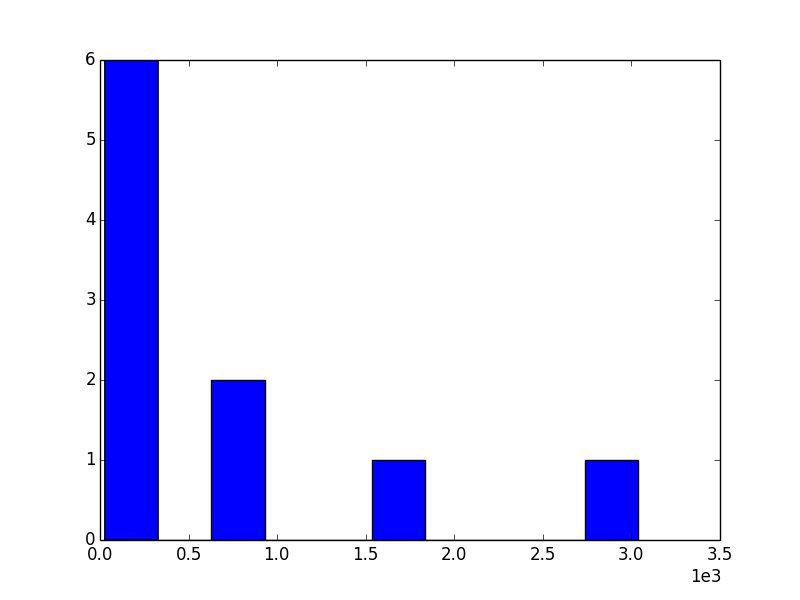
\includegraphics[width=1\linewidth]{img/histograms/fa_clustered_fa_mask_region_sizes_hist.png}
        \caption{Cluster size distribution histogram (Voxel count X Cluster count).}
        \label{subfig:fa_hist_region}
      \end{subfigure}\hfill%
      \begin{subfigure}[t]{.49\textwidth}
        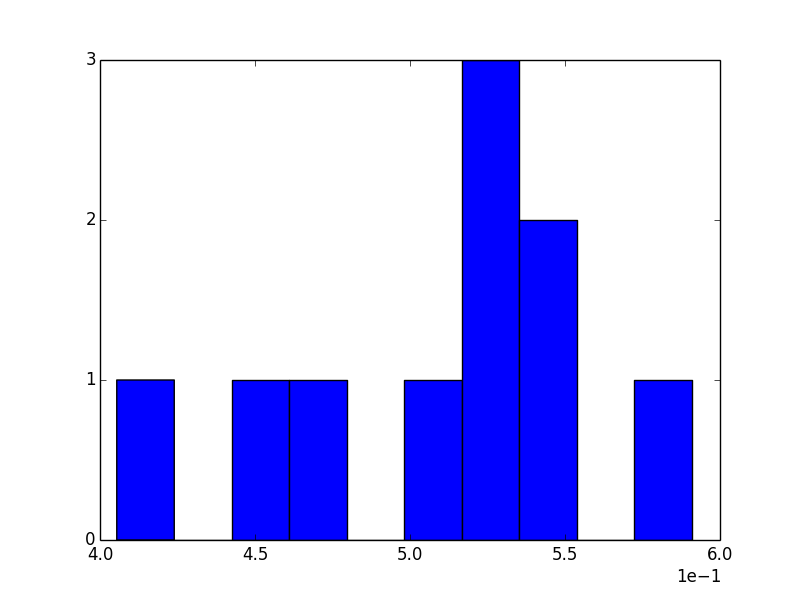
\includegraphics[width=1\linewidth]{img/histograms/fa_clustered_fa_mask_fa_means_hist.png}
        \caption{Histogram for FA mean frequency (Cluster count X FA mean).}
        \label{subfig:fa_hist_fa}
      \end{subfigure}\hfill\\
      \begin{subfigure}[t]{.49\textwidth}
        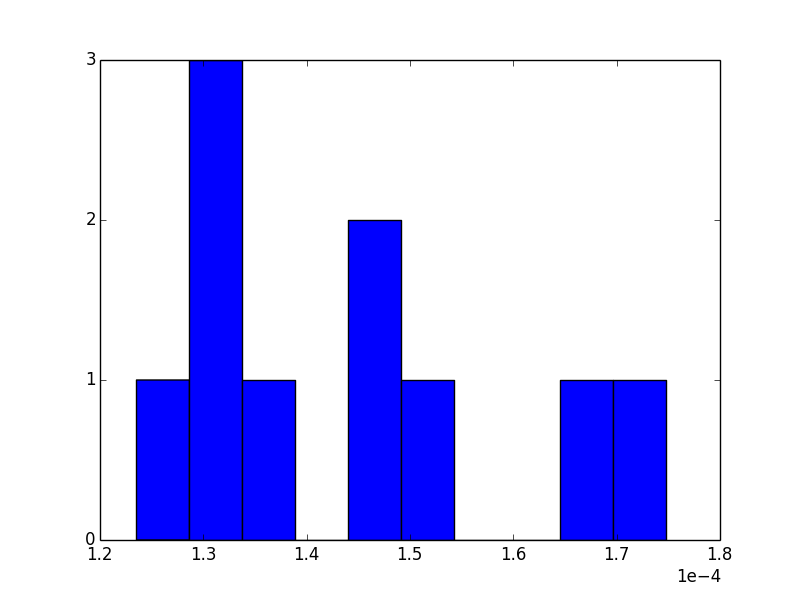
\includegraphics[width=1\linewidth]{img/histograms/fa_clustered_fa_mask_md_means_hist.png}
        \caption{Histogram for MD mean frequency (Cluster count X MD mean).}
        \label{subfig:fa_hist_md}
      \end{subfigure}\hfill%
      \begin{subfigure}[t]{.49\textwidth}
        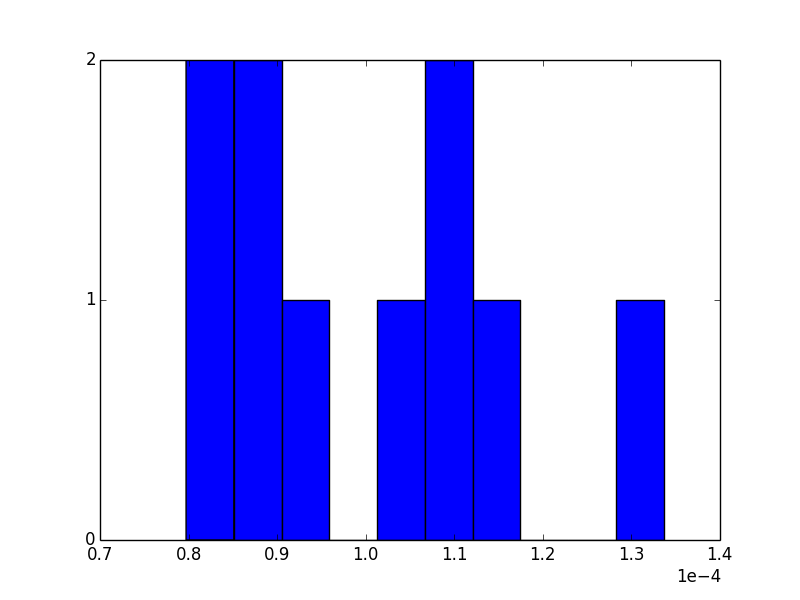
\includegraphics[width=1\linewidth]{img/histograms/fa_clustered_fa_mask_rd_means_hist.png}
        \caption{Histogram for RD mean frequency (Cluster count X RD mean).}
        \label{subfig:fa_hist_rd}
      \end{subfigure}\hfill\\
      \begin{subfigure}[t]{.49\textwidth}
        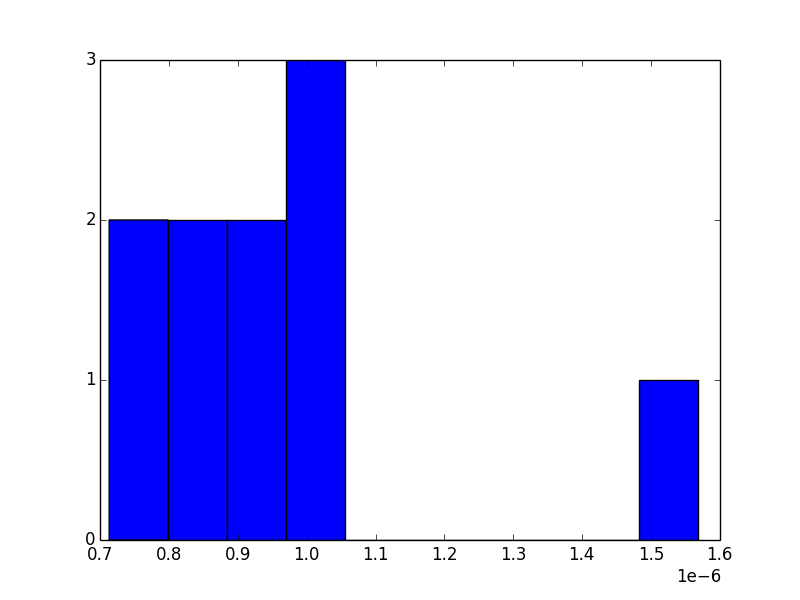
\includegraphics[width=1\linewidth]{img/histograms/fa_clustered_fa_mask_tc_means_hist.png}
        \caption{Histogram for TC mean frequency (Cluster count X TC mean).}
        \label{subfig:fa_hist_tc}
      \end{subfigure}\hfill%
      \begin{subfigure}[t]{.49\textwidth}
        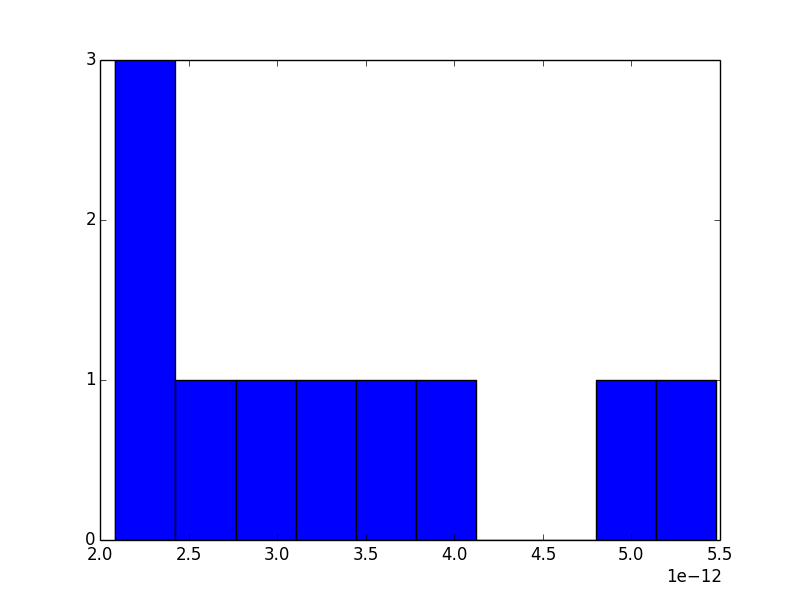
\includegraphics[width=1\linewidth]{img/histograms/fa_clustered_fa_mask_tv_means_hist.png}
        \caption{Histogram for TV mean frequency (Cluster count X TV mean).}
        \label{subfig:fa_hist_tv}
      \end{subfigure}\hfill

      \caption{Histograms for statistics distribution when clustered by FA values.}
      \label{fig:fa-histograms}
    \end{figure}

    This type of clusterization grouped voxels with FA values which don't differ no more then 0.15 (standard deviation from the entire region \ref{subsec:fa-threshold}) taking 19m32.754s\footnote{Sequential time: 13m24.782s} to get computed and another 3m18.221s\footnote{Sequential time: 3m18.922s} to generate the statistics.

    \newpage
    \subsubsection{RD}
    \begin{figure}[!ht]
      \centering

      \begin{subfigure}[t]{.49\textwidth}
        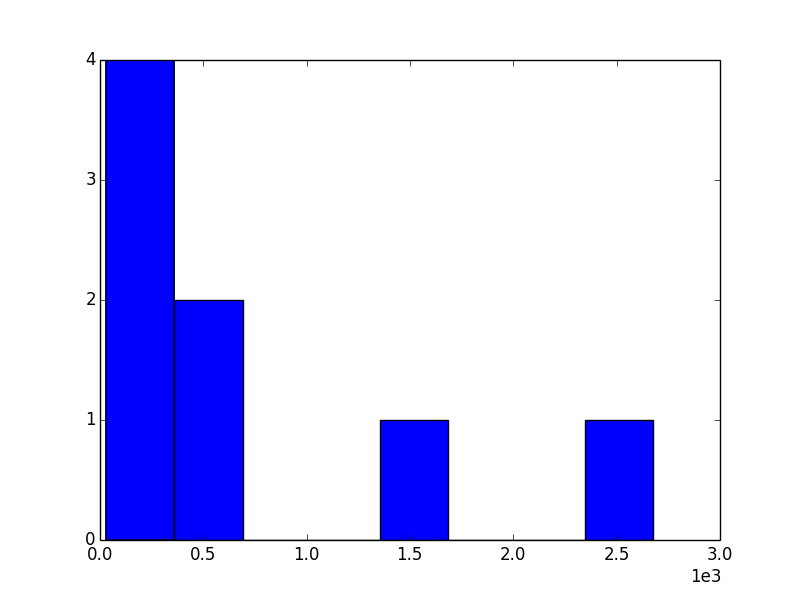
\includegraphics[width=1\linewidth]{img/histograms/rd_clustered_fa_mask_region_sizes_hist.png}
        \caption{Cluster size distribution histogram (Voxel count X Cluster count).}
        \label{subfig:fa_hist_region}
      \end{subfigure}\hfill%
      \begin{subfigure}[t]{.49\textwidth}
        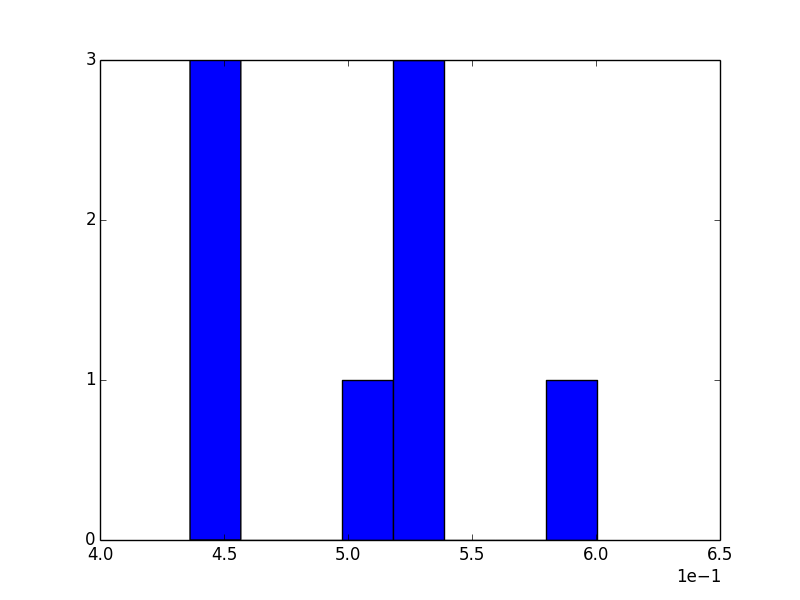
\includegraphics[width=1\linewidth]{img/histograms/rd_clustered_fa_mask_fa_means_hist.png}
        \caption{Histogram for FA mean frequency (Cluster count X FA mean).}
        \label{subfig:fa_hist_fa}
      \end{subfigure}\hfill\\
      \begin{subfigure}[t]{.49\textwidth}
        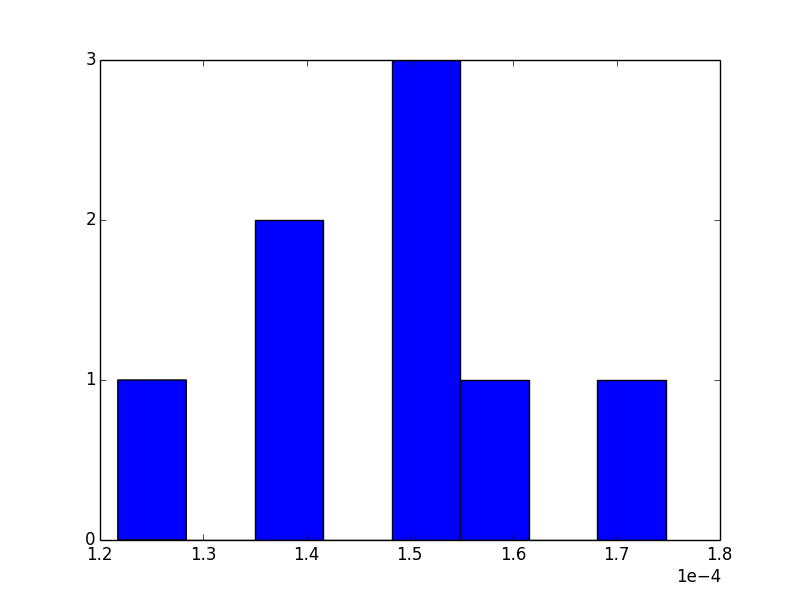
\includegraphics[width=1\linewidth]{img/histograms/rd_clustered_fa_mask_md_means_hist.png}
        \caption{Histogram for MD mean frequency (Cluster count X MD mean).}
        \label{subfig:fa_hist_md}
      \end{subfigure}\hfill%
      \begin{subfigure}[t]{.49\textwidth}
        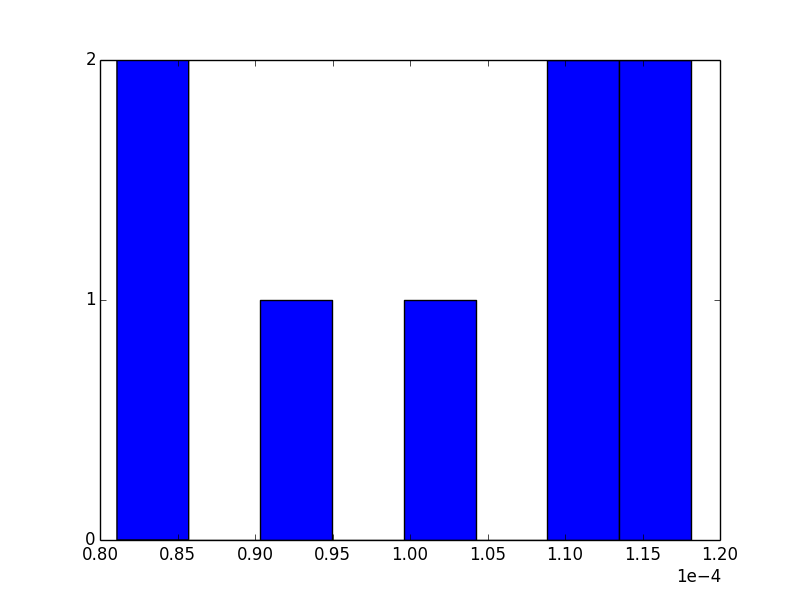
\includegraphics[width=1\linewidth]{img/histograms/rd_clustered_fa_mask_rd_means_hist.png}
        \caption{Histogram for RD mean frequency (Cluster count X RD mean).}
        \label{subfig:fa_hist_rd}
      \end{subfigure}\hfill\\
      \begin{subfigure}[t]{.49\textwidth}
        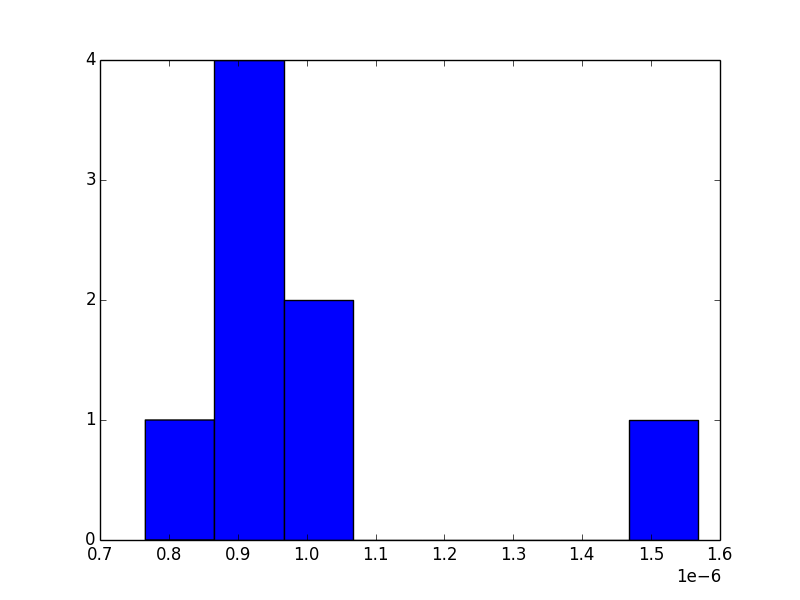
\includegraphics[width=1\linewidth]{img/histograms/rd_clustered_fa_mask_tc_means_hist.png}
        \caption{Histogram for TC mean frequency (Cluster count X TC mean).}
        \label{subfig:fa_hist_tc}
      \end{subfigure}\hfill%
      \begin{subfigure}[t]{.49\textwidth}
        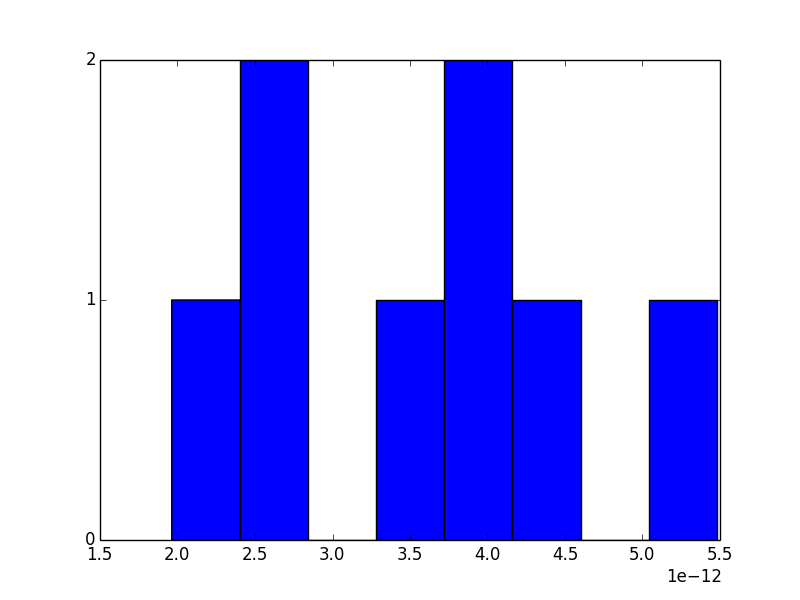
\includegraphics[width=1\linewidth]{img/histograms/rd_clustered_fa_mask_tv_means_hist.png}
        \caption{Histogram for TV mean frequency (Cluster count X TV mean).}
        \label{subfig:fa_hist_tv}
      \end{subfigure}\hfill

      \caption{Histograms for statistics distribution when clustered by RD values.}
      \label{fig:fa-histograms}
    \end{figure}

    This type of clusterization grouped voxels with RD values which don't differ no more then 0.00005 (standard deviation from the entire region \ref{subsec:fa-threshold}) taking 17m21.273s\footnote{Sequential time: 89m29.007s} to get computed and another 5m0.552s\footnote{Sequential time: 6m12.551s} to generate the statistics.

    \newpage
    \subsubsection{TC}
    \begin{figure}[!ht]
      \centering

      \begin{subfigure}[t]{.49\textwidth}
        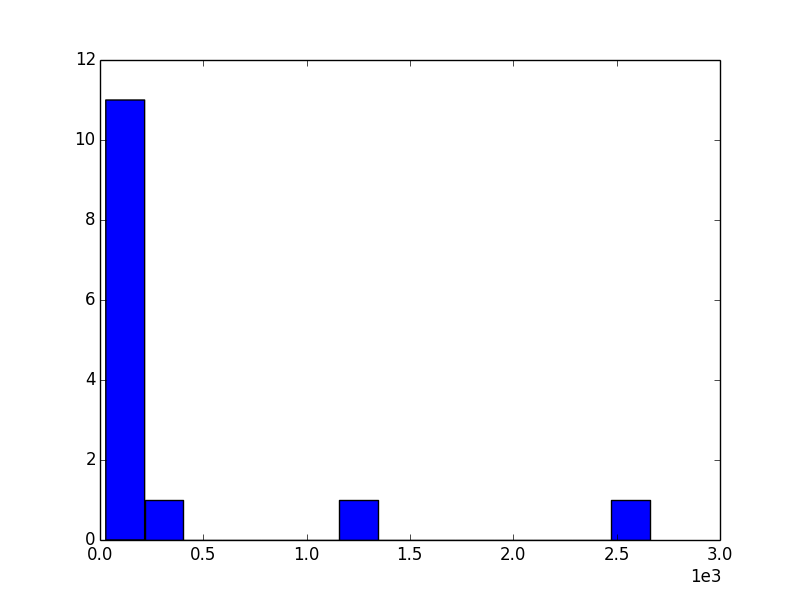
\includegraphics[width=1\linewidth]{img/histograms/tc_clustered_fa_mask_region_sizes_hist.png}
        \caption{Cluster size distribution histogram (Voxel count X Cluster count).}
        \label{subfig:fa_hist_region}
      \end{subfigure}\hfill%
      \begin{subfigure}[t]{.49\textwidth}
        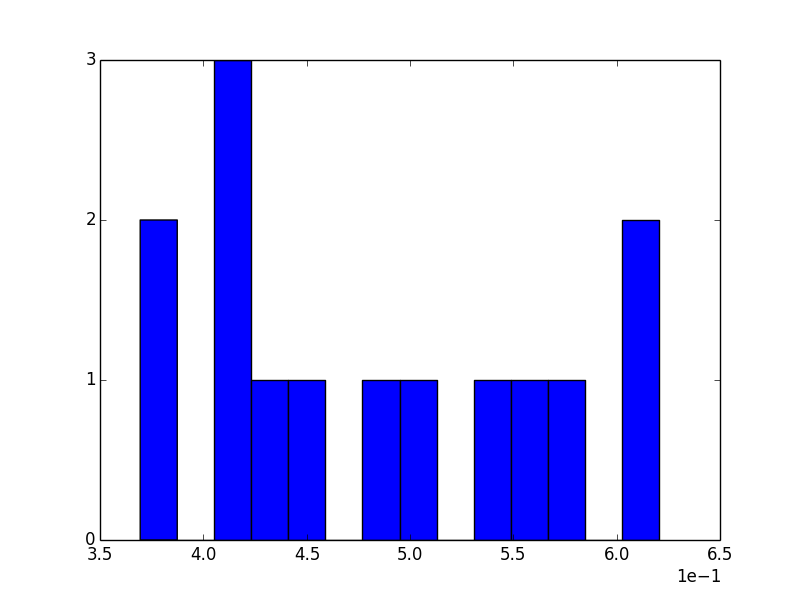
\includegraphics[width=1\linewidth]{img/histograms/tc_clustered_fa_mask_fa_means_hist.png}
        \caption{Histogram for FA mean frequency (Cluster count X FA mean).}
        \label{subfig:fa_hist_fa}
      \end{subfigure}\hfill\\
      \begin{subfigure}[t]{.49\textwidth}
        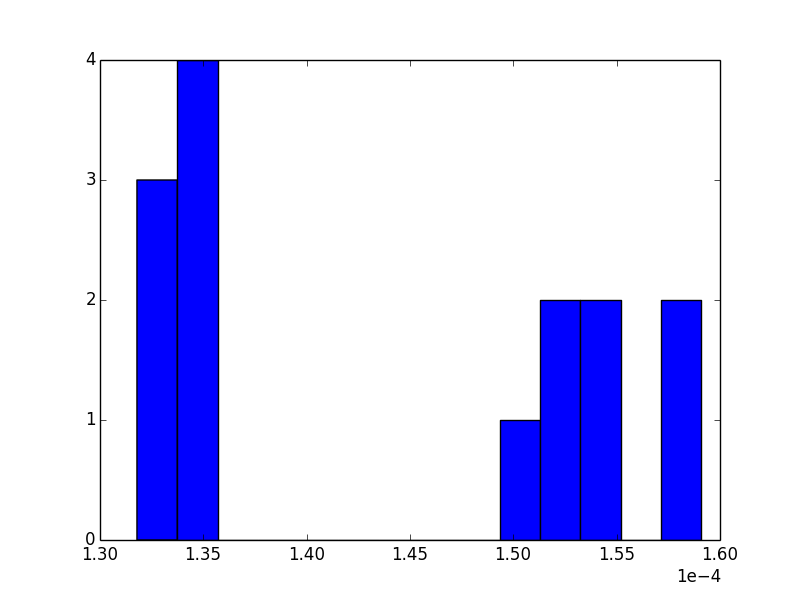
\includegraphics[width=1\linewidth]{img/histograms/tc_clustered_fa_mask_md_means_hist.png}
        \caption{Histogram for MD mean frequency (Cluster count X MD mean).}
        \label{subfig:fa_hist_md}
      \end{subfigure}\hfill%
      \begin{subfigure}[t]{.49\textwidth}
        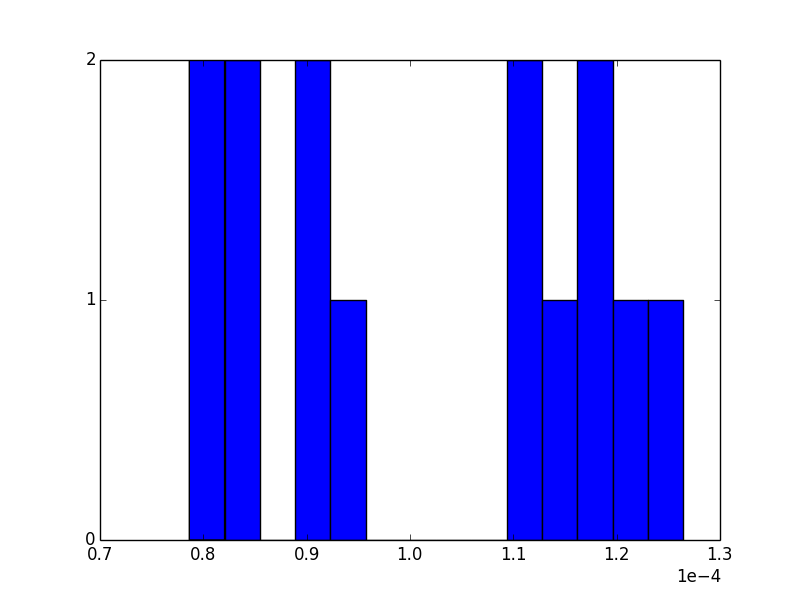
\includegraphics[width=1\linewidth]{img/histograms/tc_clustered_fa_mask_rd_means_hist.png}
        \caption{Histogram for RD mean frequency (Cluster count X RD mean).}
        \label{subfig:fa_hist_rd}
      \end{subfigure}\hfill\\
      \begin{subfigure}[t]{.49\textwidth}
        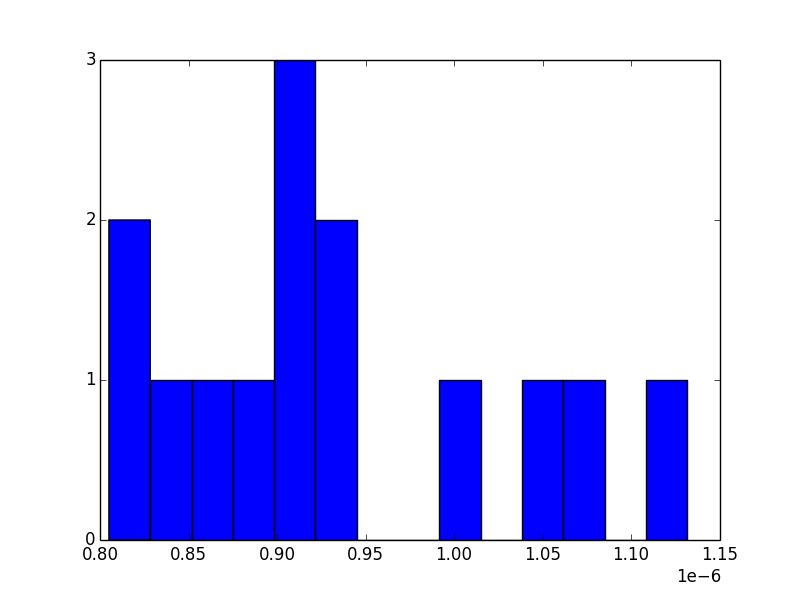
\includegraphics[width=1\linewidth]{img/histograms/tc_clustered_fa_mask_tc_means_hist.png}
        \caption{Histogram for TC mean frequency (Cluster count X TC mean).}
        \label{subfig:fa_hist_tc}
      \end{subfigure}\hfill%
      \begin{subfigure}[t]{.49\textwidth}
        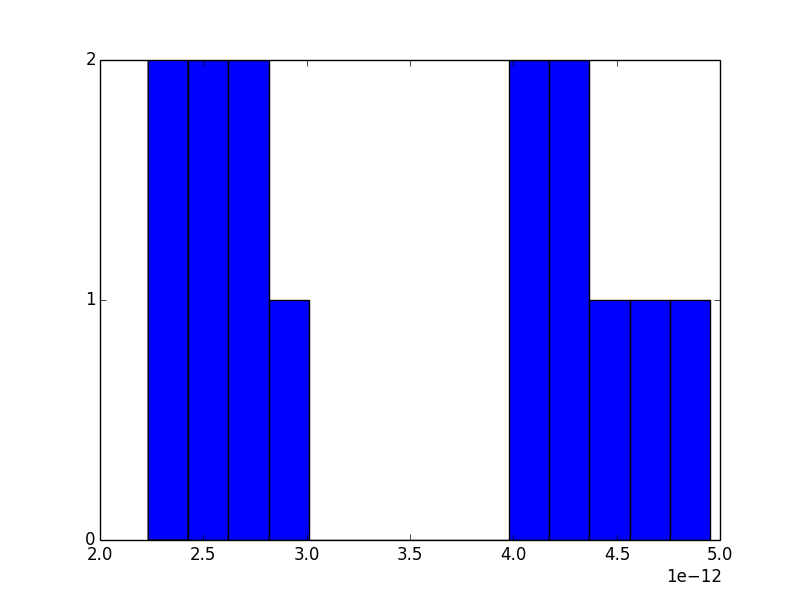
\includegraphics[width=1\linewidth]{img/histograms/tc_clustered_fa_mask_tv_means_hist.png}
        \caption{Histogram for TV mean frequency (Cluster count X TV mean).}
        \label{subfig:fa_hist_tv}
      \end{subfigure}\hfill

      \caption{Histograms for statistics distribution when clustered by TC values.}
      \label{fig:fa-histograms}
    \end{figure}

    This type of clusterization grouped voxels with FA values which don't differ no more then 0.0000005 (standard deviation from the entire region \ref{subsec:fa-threshold}) taking 62m17.542s\footnote{Sequential time: 76m56.386s} to get computed and another 4m34.027s\footnote{Sequential time: 4m11.423s} to generate the statistics.

    \newpage
    \subsubsection{TV}
    \begin{figure}[!ht]
      \centering

      \begin{subfigure}[t]{.49\textwidth}
        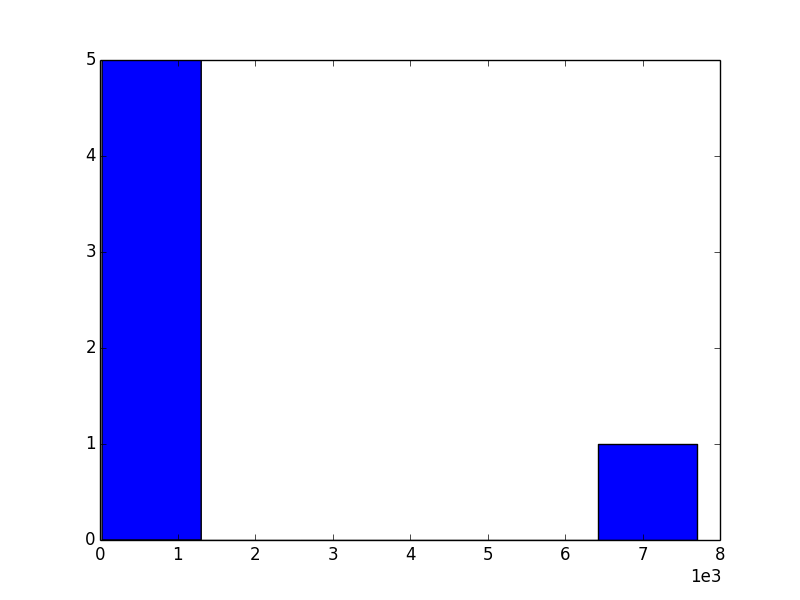
\includegraphics[width=1\linewidth]{img/histograms/tv_clustered_fa_mask_region_sizes_hist.png}
        \caption{Cluster size distribution histogram (Voxel count X Cluster count).}
        \label{subfig:fa_hist_region}
      \end{subfigure}\hfill%
      \begin{subfigure}[t]{.49\textwidth}
        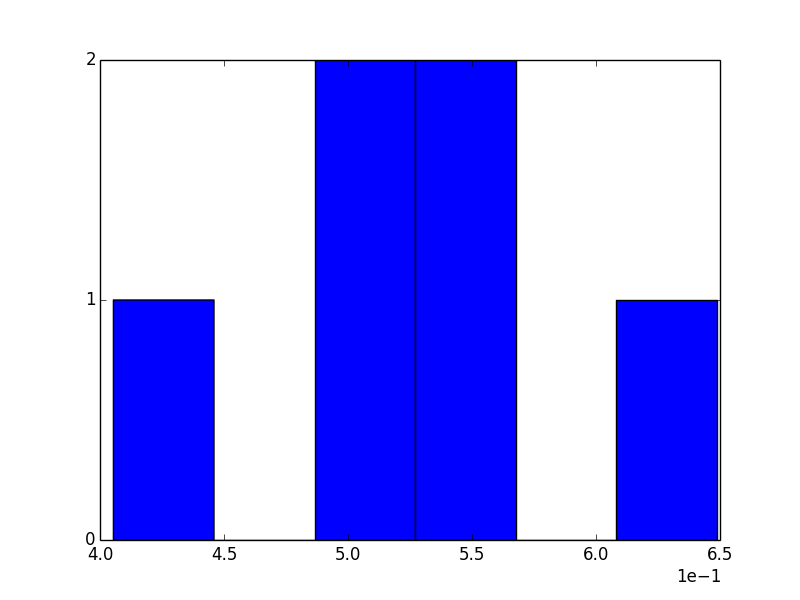
\includegraphics[width=1\linewidth]{img/histograms/tv_clustered_fa_mask_fa_means_hist.png}
        \caption{Histogram for FA mean frequency (Cluster count X FA mean).}
        \label{subfig:fa_hist_fa}
      \end{subfigure}\hfill\\
      \begin{subfigure}[t]{.49\textwidth}
        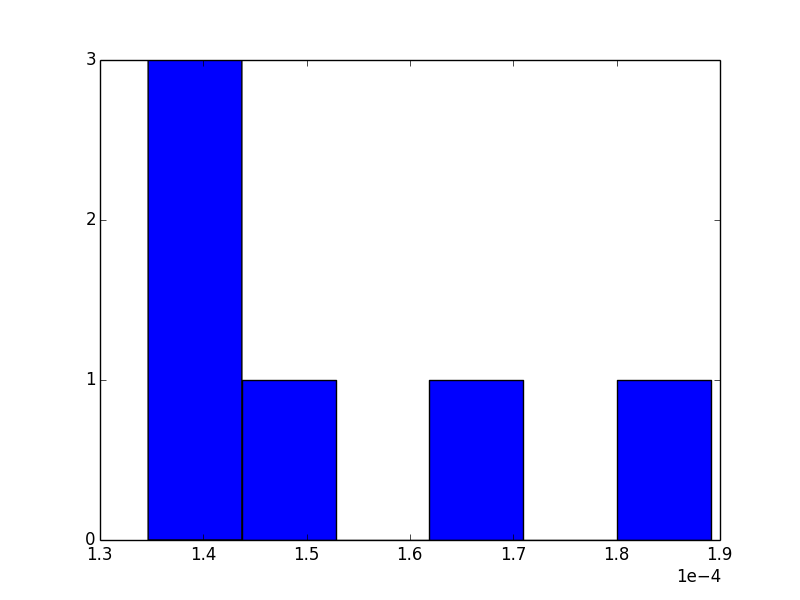
\includegraphics[width=1\linewidth]{img/histograms/tv_clustered_fa_mask_md_means_hist.png}
        \caption{Histogram for MD mean frequency (Cluster count X MD mean).}
        \label{subfig:fa_hist_md}
      \end{subfigure}\hfill%
      \begin{subfigure}[t]{.49\textwidth}
        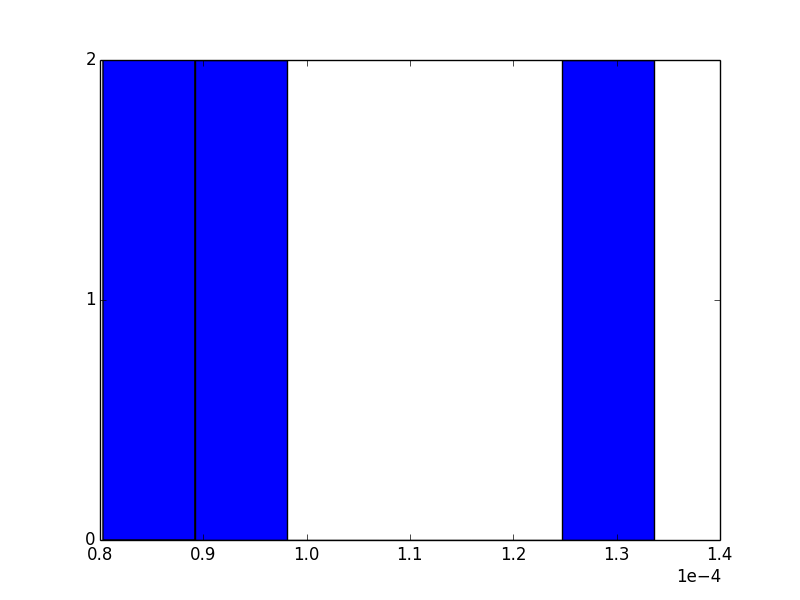
\includegraphics[width=1\linewidth]{img/histograms/tv_clustered_fa_mask_rd_means_hist.png}
        \caption{Histogram for RD mean frequency (Cluster count X RD mean).}
        \label{subfig:fa_hist_rd}
      \end{subfigure}\hfill\\
      \begin{subfigure}[t]{.49\textwidth}
        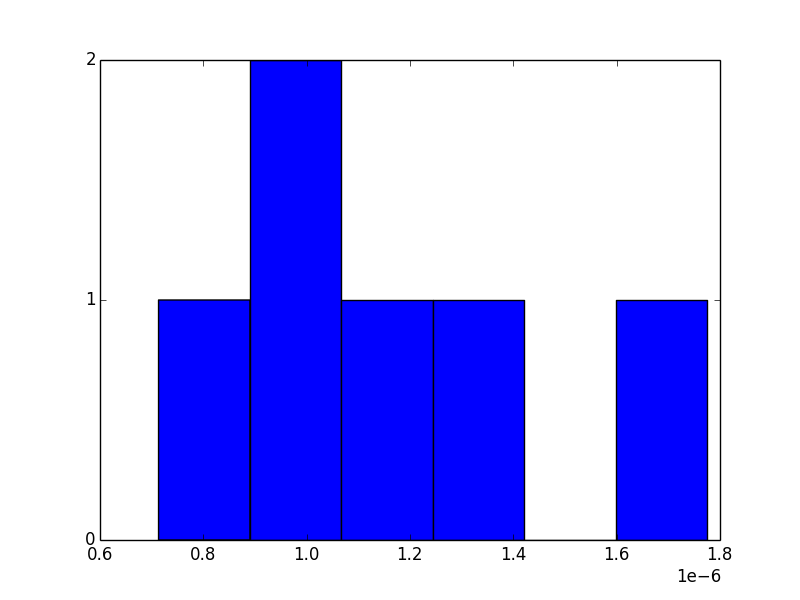
\includegraphics[width=1\linewidth]{img/histograms/tv_clustered_fa_mask_tc_means_hist.png}
        \caption{Histogram for TC mean frequency (Cluster count X TC mean).}
        \label{subfig:fa_hist_tc}
      \end{subfigure}\hfill%
      \begin{subfigure}[t]{.49\textwidth}
        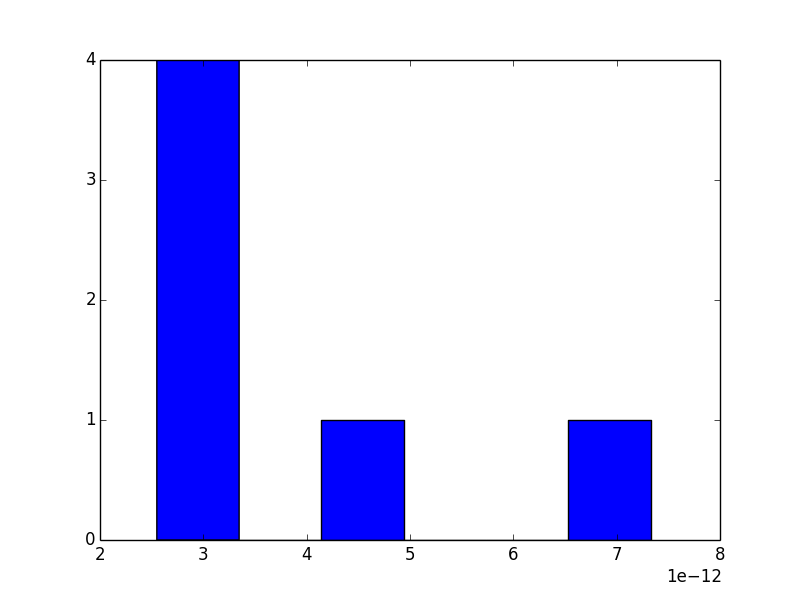
\includegraphics[width=1\linewidth]{img/histograms/tv_clustered_fa_mask_tv_means_hist.png}
        \caption{Histogram for TV mean frequency (Cluster count X TV mean).}
        \label{subfig:fa_hist_tv}
      \end{subfigure}\hfill

      \caption{Histograms for statistics distribution when clustered by TV values.}
      \label{fig:fa-histograms}
    \end{figure}

    This type of clusterization grouped voxels with FA values which don't differ no more then 0.00000001 taking 17m29.473s\footnote{Sequential time: 137m11.281s} to get computed and another 6m24.052s\footnote{Sequential time: 5m38.443s} to generate the statistics.

\chapter{Conclusion}

\end{document}